%!TEX encoding = IsoLatin

%% Document is article 
\documentclass[a4paper]{article}

%% ----------------------------------------------------- PACKAGES ----------------------------------------------------- %%
\usepackage{coolArticle}
\usepackage{algorithm2e}


%% ---------------------------------------------------- DOCUMENT ---------------------------------------------------- %%
\begin{document}

	\titlebox{0.4}{Feed Forward Neural Networks}{and how to train them}
	
		
	\vhrulefill{2pt}
	
	\tableofcontents
	
	\vhrulefill{2pt}
	
	\section{Feed Forward Neural Network}
	{
		\paragraph{} Recall the basic model for regression and classification tasks : 
		\begin{equation}
			y(w,x) = f\left(\sum_iw_i\phi_i(x)\right)
		\end{equation}
		where $f$ is called the activation function. \newline
		With neural networks, our goal is to extend this model to basis function that can be parametrizable. Each basis function is itself a non-linear function of a linear combination of the inputs, where the combination weights are adaptable parameters. 
		
		\subsection{The basic feed-forward neural network}
		{
			\paragraph{} Such considerations lead to the most basic neural network model. Let us define the following : 
			\begin{equation}
				\forall{j}\in\{1,\hdots,M\}, \quad a_j = w_{j0}^{(1)} + \sum_{i=1}^D w_{ji}^{(1)}x_i 
			\end{equation}
		The scalars $(a_j)_{j\in\{1,\hdots,M\}}$ are called {\textcolor{red}{activations units}}. They are transformed using a \emph{differentiable}, usually non-linear activation function : 
		\begin{equation}
			\forall{j}\in\{1,\hdots,M\}, \quad z_j = h(a_j)
		\end{equation}
		The activation function $h(.)$ is usually chosen to a sigmoid function such as the logistic sigmoid or the tanh(.) function. 
	
		\paragraph{} In the context of neural networks, the $(z_j)_j$ correspond to the output of the initial basis functions are called the \emph{output of the hidden units}. They are therefore linearly mixed to produce the {\textcolor{red}{output unit activations}} : 
		\begin{equation}
			\forall{k}\in\{1,\hdots,K\}, \quad a_k = w_{k0}^{(2)} + \sum_{j=1}^M w_{kj}^{(2)}z_j
		\end{equation}
		The network's output is then computed b applying an output activation function : 
		\begin{equation}
			\forall{k}\in\{1,\hdots,K\}, \quad y_k = h(a_k)
		\end{equation}
		
		\paragraph{} The process we just described to compute both the hidden layer activations, the hidden layer output, the output unit activations and the networks output is called \textbf{\textcolor{red}{feedforward propagation}}. It is the basis of feed-forward net, which topology can be summed un by figure (\ref{feed_forward_topo}). 
		
		\begin{figure}[h!]
			\begin{center}
				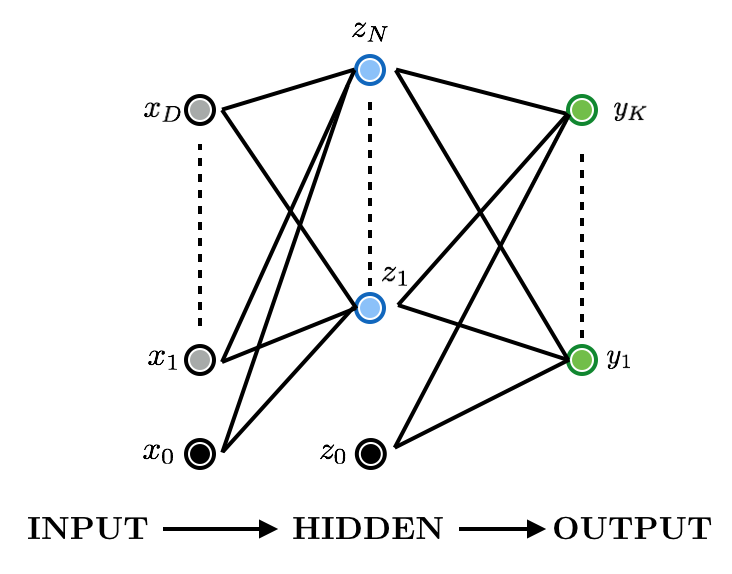
\includegraphics[width=0.5\linewidth]{nn_ff_topo}
				\caption{Topology of a neural network with one hidden layer}
				\label{feed_forward_topo}
			\end{center}
		\end{figure}
		
		\paragraph{} Of course, one can decide to stack as many hidden layer as he wants. The resulting neural net is therefore called a \emph{deep} neural net, performing \emph{deep learning}. 
		}	
		
		\subsection{Activation function}
		{
			\paragraph{} Activation functions for the hidden and output layers highly depend on the task that the neural net is performing. For standard regression problems, linear activation or rectified linear activation functions are preferred. For binary classification, the logistic function is the most common activation function : 
			\begin{equation}
				\sigma(a) = \frac{1}{1+e^{-a}}
			\end{equation}
			For multi-class problems, the softmax function is the most reasonable choice : 
			\begin{equation}
				\text{softmax}(z) = \left(\frac{e^{z_j}}{\sum_k e^{z_k}} \right)_j
			\end{equation}
		}
		\subsection{The network's output}
		{
			Assuming that the output activation function is a logistic sigmoid, the output takes the form of a non-linear function of the inputs :  
			\begin{equation}
				\forall{k}\in\{1,\hdots,K\}, \quad y_k = \sigma\left( \sum_{j=1}^M w^{(2)}_{kj}h\left(\sum_{i=1}^D w_{ji}^{(1)} + w_{j0}^{(1)}\right) + w^{(2)}_{k0}\right)
			\end{equation}
			which can be simplified by adding a dimension to the input to absorb the bias into a mock dimension : 
			\begin{equation}
				\forall{k}\in\{1,\hdots,K\}, \quad y_k = \sigma\left( \sum_{j=0}^M w_{kj}^{(2)}h\left(\sum_{i=0}^D w_{ji}^{(1)} x_i\right)\right)
			\end{equation}
			
			\paragraph{} The approximation abilities of feed-forward networks have been widely studied. Feed-forward artificial neural networks are said to be \emph{general approximators}. Indeed, it was shown that a two-layer network with linear output can uniformly approximate any continuous functions on a compact input domain to arbitrary accuracy, given that the hidden layer has a sufficient large number of units. The remaining questions is how to tune the parameters (i.e the weights) in order to achieve any given accuracy for a function approximation ?
		}
	}
	
	\section{Network training}
	{
		\paragraph{} We consider a dataset $\mathcal{X} = \left\{ x_1, \hdots, x_n\right\}\in\left( \mathbb{R}^D\right)^N$, with a corresponding set of target vectors $\mathcal{T} = \left\{t_1,\hdots, t_N\right\}$. 
		
		\subsection{Error function}
		{
			\paragraph{} As with other machine learning algorithm, we are going to train our network by minimizing an error function that represent how well the network approximate the underlying function sampled at the dataset's points. 
			
			\subsubsection{Regression task}
			{
				\paragraph{} For regression tasks, a commonly used error function is the \emph{sum of square} error function : 
				\begin{equation}
					E(w,\mathcal{X},\mathcal{T}) = \sum_{n=1}^N \lVert y(x_n,w) - t_n\rVert ^2 
				\end{equation}
				As with many different model, this error function can be motivated by a probabilistic approach. Let us assume that the real-valued target are Gaussian distributed around an $x$-dependent mean. Therefore $\forall{n}\in\{1,\hdots, N \}$ : 
				\begin{equation}
					\condp{t_n}{\mathcal{X},w} = \normalDb{t_n}{y(x_n,w)}{\beta^{-1}}
				\end{equation}
				where $\beta$ is known as the distribution's \emph{precision}. Therefore assuming independence between the drawn samples, we have that : 
				\begin{equation}
					\condp{\mathcal{T}}{\mathcal{X},w} = \prod_{n=1}^N  \normalDb{t_n}{y(x_n,w)}{\beta^{-1}}
				\end{equation}
				and 
				\begin{equation}
					-\log{\left[ \condp{\mathcal{T}}{\mathcal{X},w} \right]} = cste + \frac{\beta}{2} \sum_{n=1}^N \left\{ y(x_n,w) - t_n\right\}^2
				\end{equation}
				Therefore a \emph{maximum-likelihood} solution, which will try to maximize the likelihood of the dataset, is given by minimizing the sum-of-square error function. This approach is adapted to regression problem, but can lead to slow learning in case of sigmoid activation function. For binary classification tasks (where the common approach is logistic regression), there exists a more natural error function, which is not the victim of slow learning far from correctness. 
			}
			\subsubsection{Binary classification task}
			{
				\paragraph{} We now consider the case of binary classification. Let's consider a logistic sigmoid output activation function. Therefore, the network output can be interpreted as the condition probability $p\left(\mathcal{C}_1\vert  x\right)$. The conditional distribution of the targets given the inputs is therefore a Bernouilli distribution of the form : 
				\begin{equation}
					\condp{t}{x,w} = y(x,w)^t \{1-y(w,x)\}^{1-t}
				\end{equation}
				The derivation of the error function is performed as in the regression task. We obtain the \textcolor{red}{cross-entropy function} : 
				\begin{equation}
					E(w,\mathcal{X},\mathcal{T}) = -\sum_{n=1}^N \left[ t_n\log{y_n} + (1-t_n)\log{(1-y_n)}\right]
				\end{equation}
				
				\paragraph{} The real benefit of this error function is that it avoid slow learning that can appear with the sum-of-square error function (computes the derivatives with respect to $w$ when there is misclassification .. ). 
				
				\paragraph{} The same reflexion with the standard multi-class problem (Multinouilli distribution) leads to the following error function : 
				\begin{equation}
					E(w,\mathcal{X},\mathcal{T}) = -\sum_{n=1}^N \sum_{k=1}^K t_{nk}\log{y_k(x_n,w)}
				\end{equation}
			}
		}
		\subsection{Network optimization}
		{
			\paragraph{} Of course, for complex neural network, analytical solving of the optimization problem : 
			\begin{equation}
				\max_w E(w,\mathcal{X},\mathcal{T})
			\end{equation}
			is untractable. We therefore need to use sequential optimization algorithms (steepest descent, Newton or quasi-Newtons methods). 
			
			\paragraph{} The offline optimization can be quite costly for larget dataset. Indeed, if one decide to run a finite difference gradient optimization, he must run $2*W^2$ feed-forward operations !.) Fortunately, there exist an on-line version of gradient descent that is very helpful for large datasets. Since : 
			\begin{equation}
				E(w) = \sum_{n=1}^N E_n(w) 
			\end{equation}
			one can follow the update rule given by : 
			\begin{equation}
				w^{(\tau+1)} = w^{(\tau)} - \eta \nabla E_n(w^{(\tau)})
			\end{equation}
			This update rule is known as the \textcolor{red}{stochastic gradient descent}. It is repeated by cycling through the date (usually with replacement). One can also decide to pack datapoints into small group and then perform optimization on this small part of the data, which is called \emph{mini-batch} gradient descent. Such methods display better handling of data redundancy and can escape from local minima the batch method would get trapped in (a local minima for the whole dataset is not mandatorily a local minima for one datapoint). 
		}
	}
	
	\section{The backpropagation algorithm}
	{
		\paragraph{} Now that we now how to train our network using variational informations, we need to compute such variations (gradient, Jacobian, Hessian). If all of those can of course be computed via finite difference, those methods are numerically needy. We hereinafter describe the \emph{back-propagation} algorithm, which introduce an efficient way to compute gradient informations. 
		
		\paragraph{} We consider a neural network having arbitrary feed-forward topology, arbitrary differentiable activations functions. 
		
		\paragraph{} For the sake of the example, we consider an error function that can be written as a sum of terms errors, one for each datapoint : 
		\begin{equation}
			E(w,x) = \sum_n E_n(w)
		\end{equation}
		We'll therefore focus on computing $\nabla E_n(w)$. 
		
		\paragraph{} Let us first consider the simplest linear model 
		\begin{equation}
			y_k = \sum_i w_{ki}x_i
		\end{equation}
		along with the error function : 
		\begin{equation}
			E_n(w,\mathcal{X},\mathcal{T}) = \frac{1}{2}\sum_n\{ y_n - t_n \}^2
		\end{equation}
		Therefore we'll have that : 
		\begin{equation}
			\frac{\partial E_n}{\partial w_{ji}} = (y_{nj} - t_{nj})x_{ni}
		\end{equation}
		and a similar formule arises for a sigmoidal activation function. 
		
		\paragraph{} Let us now consider computing $\frac{\partial E_n}{\partial w_{ji}}$ for a link from the hidden layer to the output activation layer. By applying the cain rule : 
		\begin{equation}
			\begin{aligned} 
				\frac{\partial E_n}{\partial w_{ji}} &= \frac{\partial{E_n}}{\partial a_j}\frac{\partial a_j}{\partial w_{ji}}\\
									          &= \delta_j \frac{\partial a_j}{\partial w_{ji}} \text{ with } \delta_j = \frac{\partial{E_n}}{\partial a_j} \\
									          &= \delta_j z_i
			\end{aligned}	
		\end{equation}	  
			As we saw before, we have $\delta_k = y_k - t_k$ for a canonical output activation function. \newline
			To evaluate $\delta$'s for all units, we make use of the chain rule again : 
			\begin{equation}
				\delta_j = \sum_{k} \frac{\partial{E_n}}{\partial a_k}\frac{\partial a_k}{\partial a_j}
			\end{equation}
			for all $k$ unit to which $j$ sends a connection. 
			Therefore we obtain the \textbf{\textcolor{red}{backprop formula}} : 
			\vspace{10pt}
			
			\coolbox{white}{\textcolor{black}{Backprop formula}}
			{
				\begin{equation}
					\delta_j = h'(a_j)\left( \sum_k \delta_k w_{kj}\right)
				\end{equation}
			}
			
			\paragraph{} The full backpropagation algorithm is given below : 
			\vspace{10pt}
			
			\coolbox{white}{\textcolor{blue}{The Error Backpropagation Algorithm}}
			{
				1. Apply a datapoint $x_n$ to the network and forward propagate the input, to compute the activations of the hidden and output units. \newline
				2. Evaluate the $\delta_k$'s for the output layer unit. \newline
				3. Backpropagate the $\delta_k$'s using the backprop formula : 
				\begin{equation}
					\delta_j = h'(a_j)\left( \sum_k \delta_k w_{kj}\right)
				\end{equation}
				4. Compute $\displaystyle\frac{\partial E}{\partial w_{ji}}$ using : 
				\begin{equation}
					\frac{\partial E}{\partial w_{ji}} = \delta_j h(a_i)
				\end{equation}
				}
				
				\paragraph{} For batch-methods, the total error derivatives is given by summing over the dataset : 
				\begin{equation}
					\nabla E(w) = \sum_n \nabla E_n(w)
				\end{equation}
				
				\paragraph{} The efficiency of the backprop algorithm is $O(W)$ against $O(W^2)$ for finite differences, hence justifying its use especially for large neural networks. 
	}

\end{document}